\newpage
\section{Dashboard}
Das Dashboard soll dem Nutzer schnell und einfach die Übersicht über seine 
eigenen abonnierten Services bieten (Compute,Storage,Network).
Dabei soll auf eine Anzahl von Cloud Anbietern angeboten werden, sowohl Public 
Cloud(z.B.: AWS, Google Cloud, Azure, Digitalocean), wie auch Private Cloud (z.B.:CloudStack.Open 
Stack).
Die nachfolgenden Mockups sollen bereits einen ersten Eindruck der 
möglichen Funktionalitäten des Dashboard geben.
\\
\textbf{Beim Login wird zwischen Nutzern und Administrator unterschieden.}

\subsection{Homescreen Nutzer}
Der Nutzer kriegt eine Übersicht über die vorhanden Cloud Anbieter und kann 
gemäss Wunsch den richtigen wählen.
\begin{figure}[!htbp]
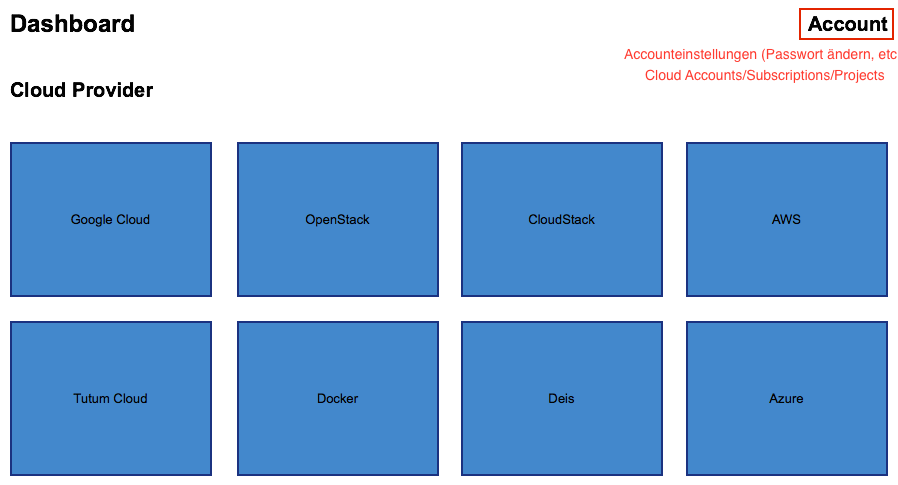
\includegraphics[width=\textwidth]{./03_Analyse/03_Dashboard/images/homescreen_user}
\caption{Homescreen Nutzer}
\end{figure}

\newpage

\subsection{Homescreen Admin}

Der Administrator kriegt lediglich eine Übersicht über die vorhanden Nutzer und 
kann diese löschen oder ändern.
\begin{figure}[!htbp]
  
\includegraphics[width=\textwidth]{./03_Analyse/03_Dashboard/images/homescreen_admin}
  \caption{Homescreen Admin}
\end{figure}


\subsection{Offerings}
Sobald man einer der Cloud Anbieter gewählt hat (auf dem Homescreen) öffnet 
sich das jeweilige Dashboard des Anbieters mit dessen spezifischen Services.
\begin{figure}[!htbp]
  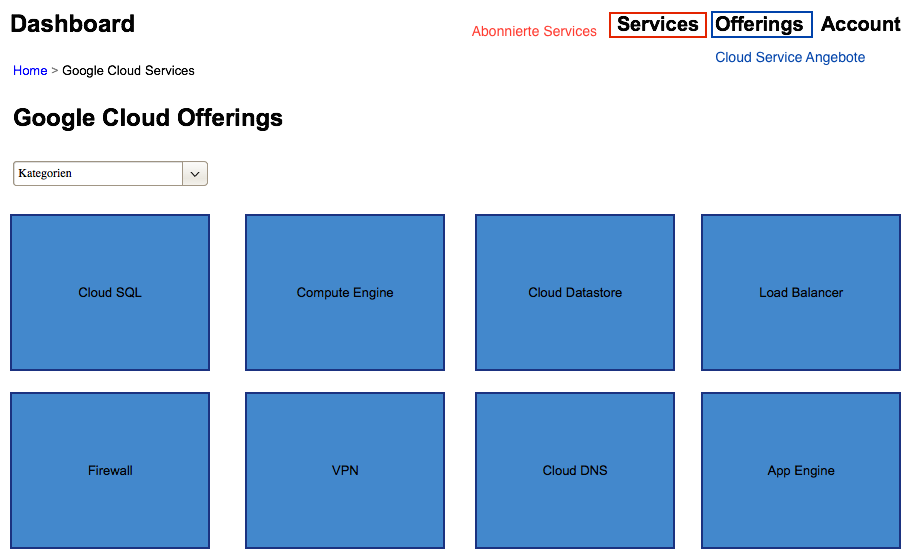
\includegraphics[width=\textwidth]{./03_Analyse/03_Dashboard/images/homescreen_google}
  \caption{Homescreen Google}
\end{figure}

\newpage

   \subsubsection{Compute:}
Hier werden nur Compute Offerings angezeigt z.B.: App Engine, Compute Engine, 
Container Engine, EC2 etc., können nach Anbieter variieren

\begin{figure}[!htbp]

   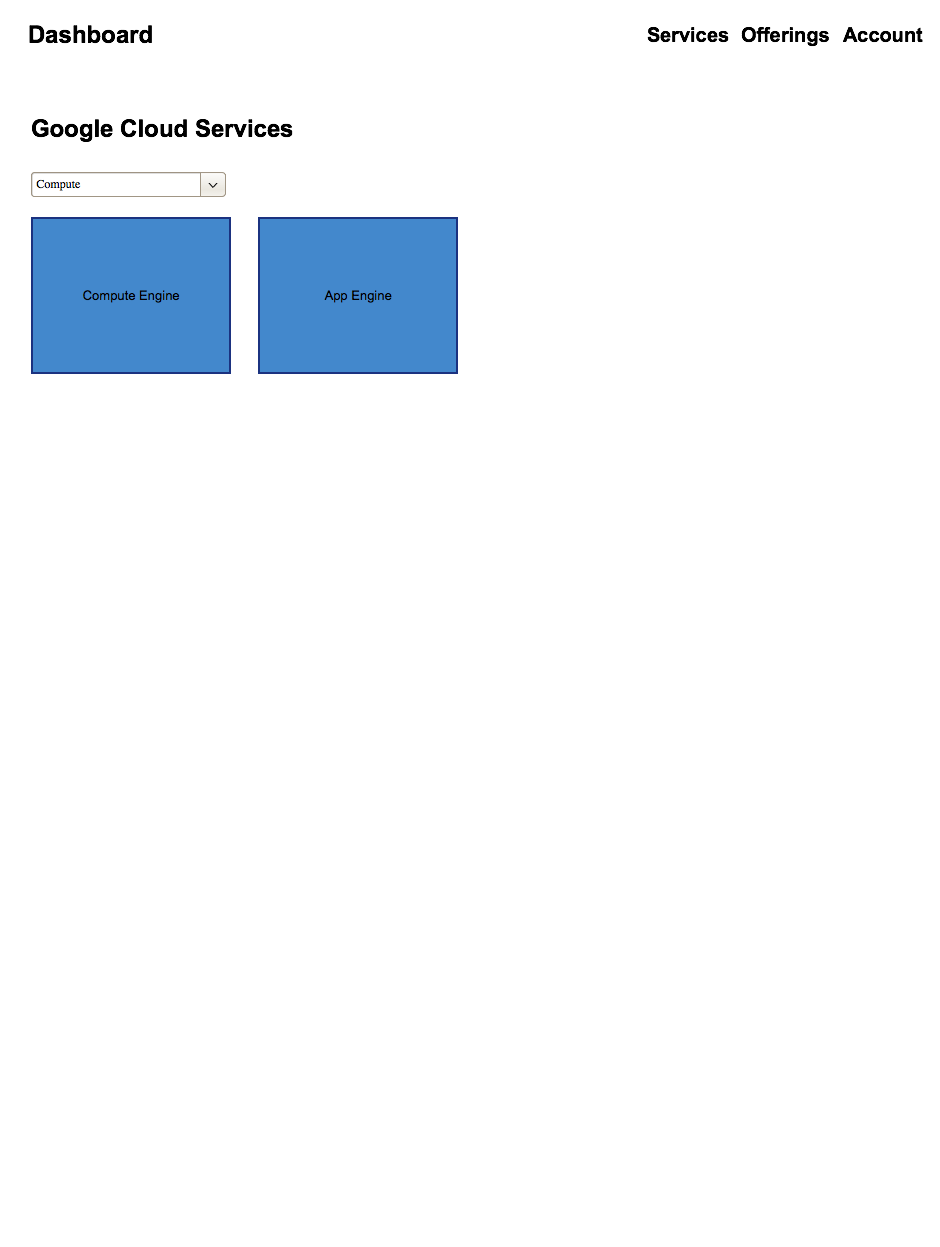
\includegraphics[width=\textwidth]{./03_Analyse/03_Dashboard/images/homescreen_google_compute}
   \caption{Homescreen Kategorie Compute}
\end{figure}
 

\subsubsection{Storage:}

Nur Storage spezifische Offerings anzeigen z.B.: Cloud Datastore, Cloud SQL, 
Cloud BigTable), die sich je nach Anbieter ändern. 
\begin{figure}[!htbp]
 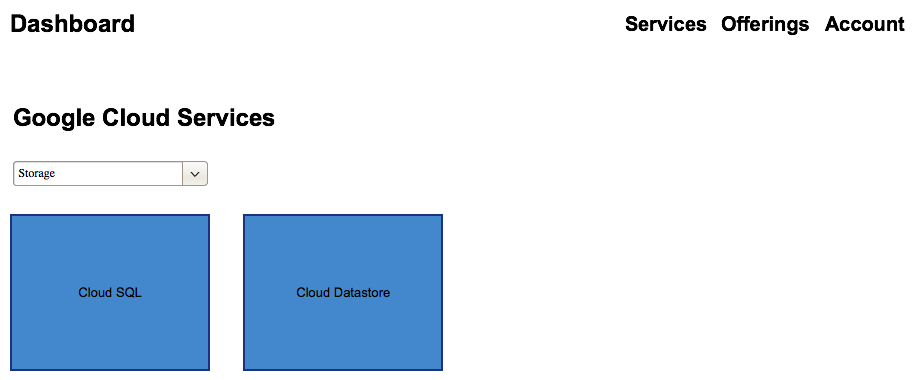
\includegraphics[width=\textwidth]{./03_Analyse/03_Dashboard/images/homescreen_google_storage}
  \caption{Homescreen Kategorie Storage}
\end{figure}

\subsubsection{Network:}
Network spezifische Offerings anbieten (Firewall, VPN, Netzwerke, Cloud DNS etc.) 
und dann verändert sich die Auswahl auch Anbieter spezifisch. 

\begin{figure}[!htbp]
 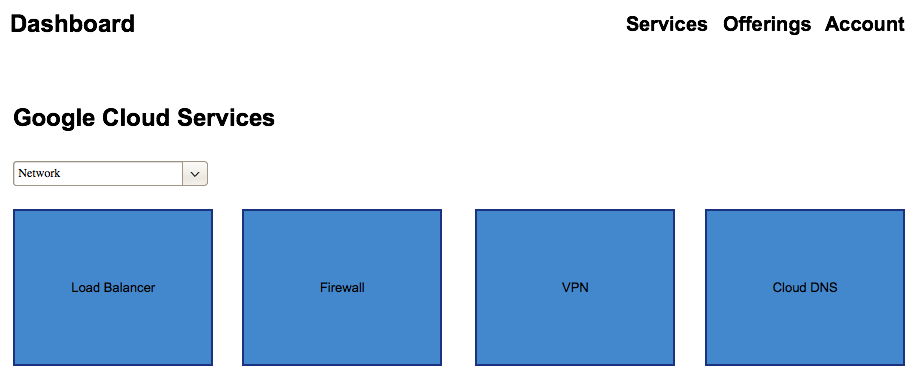
\includegraphics[width=\textwidth]{./03_Analyse/03_Dashboard/images/homescreen_google_network}
    \caption{Homescreen Kategorie Network}
\end{figure}

\newpage

\subsection{Services}
In Services kriegt man einen Überblick über all seine abonnierten Services des jeweiligen 
Anbieters und kann den zu bearbeitenden wählen.
\begin{figure}[!htbp]

\includegraphics[width=\textwidth]{./03_Analyse/03_Dashboard/images/services_overview}
\caption{Services Übersicht}
\end{figure}

\subsubsection{Compute}
Wenn man einen Compute Service wählt kriegt man eine Übersicht des Services, 
welcher Storage, Leistung + Region (Storage und Compute werden jedoch 
meistens vorgegeben durch die Instanzgrössen) + werden die Kosten pro 
Monat angezeigt.
Im Management kann dann die Instant direkt neugestartet/heruntergefahren oder gelöscht 
werden + sollen noch Links (Ip etc.) zur Verfügung stehen um sich auf die Instanz 
 verbinden zu können.
 
\begin{figure}[!htbp]
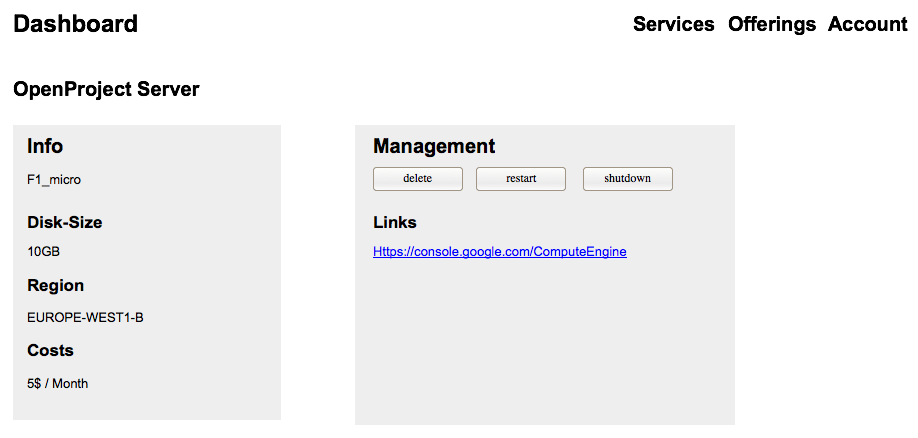
\includegraphics[width=\textwidth]{./03_Analyse/03_Dashboard/images/service_info_compute}
\caption{Services Infos Compute}
\end{figure}

\subsubsection{Storage}
Bei Storage spielt es wieder eine Rolle was für eine Art Storage es ist in 
diesem Beispiel ist es eine Cloud SQL Datenbank.
Dabei wird vielmals anhand der Anzahl Rows oder Grösse der Datenbank abgerechnet 
+ sollen hier auch wieder Links verfügbar sein, um auf ein Datenbankdashboard zu 
gelangen + die Möglichkeit geben den Service löschen zu können.

\begin{figure}[!htbp]
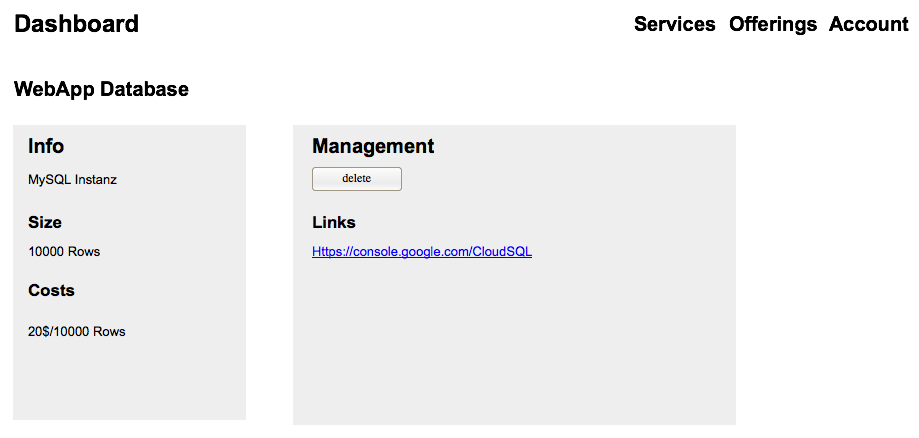
\includegraphics[width=0.8\textwidth]{./03_Analyse/03_Dashboard/images/service_info_storage}
\caption{Services Infos Storage}
\end{figure}

\subsubsection{Network}
Bei Network kann man noch einige Dinge konfigurieren von Cloud DNS bis zu 
Netzwerken (Subnetze etc.) auch Firewall Regeln, da bei den Cloud Anbietern 
vielmals nur SSH und HTTP/S zugelassener traffic ist muss man schliesslich auch 
die Möglichkeit haben Firewall Regeln festlegen zu können.
Das könnte Schlussendlich in etwa so aussehen:

\begin{figure}[!htbp]
  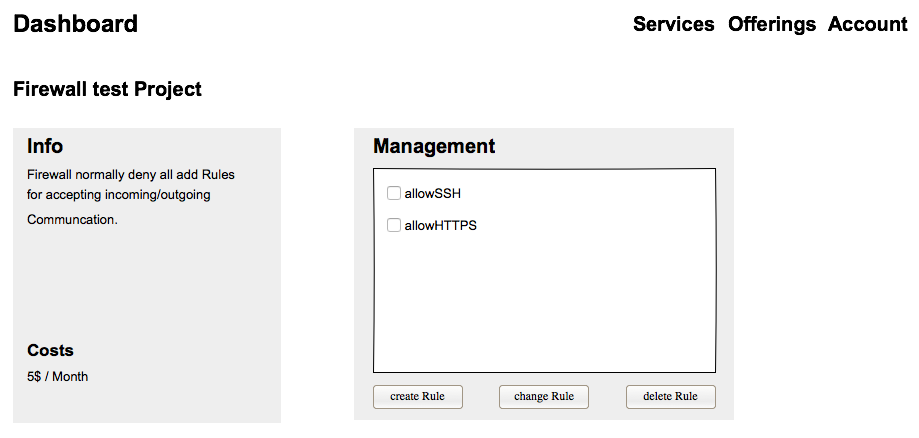
\includegraphics[width=0.8\textwidth]{./03_Analyse/03_Dashboard/images/service_info_network}
  \caption{Services Infos Network}
\end{figure}

\newpage

\subsection{Accounts/Subscriptions/Projects/...}
Für jeden Anbieter soll dem User eine Übersicht über die 
Account/Subscriptions/Projects gegeben werden, dadurch vereinfacht sich die 
Handhabung von mehreren Accounts und alle sind in einem Dashboard zusammengefügt 
(-> Security beachten).
Dadurch hat man immer den Überblick für welches Projekt/Account man wie viele 
Services abonniert hat.

\begin{figure}[!htbp]

\includegraphics[width=\textwidth]{./03_Analyse/03_Dashboard/images/account_projects.png}
\caption{Accounts Übersicht}
\end{figure}

\section{Security}
Wie bei Bitnami wäre es wohl sicherer die Zugriffsdaten für die Cloud Anbieter 
abzusichern (bei Bitnami wird dies über ein Vault sichergestellt), ansonsten 
könnte ein Angreifer ganze Instanzen bei verschiedenen Anbietern löschen oder 
sonstige Bösartige Absichten ausüben.

Dieser Vault soll auch durch ein zusätzliches Passwort geschützt sein und 
wird symmetrisch verschlüsselt (Mail Anbieter: Proton Mail\autocite{proton} macht dies ebenfalls 
so) -> jedoch fragt Bitnami bei jedem login wieder nach dem Passwort und 
vergisst dann wieder alle Instanzen (ein Abgleich mit dem Anbieter wäre hier sicher nicht 
schlecht).

\newpage

\section{Fazit}
Das Servicedashboard scheint soweit umsetzbar zu sein, ein Knackpunkt wird 
einfach noch die Absicherung der Zugriffe auf alle die Cloud Anbieter und deren 
Services.
Z.B.: Bitnami bietet ein Download für Private Key und Putty Key File an:
\begin{figure}[!htbp]
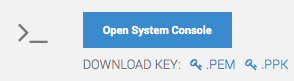
\includegraphics[width=0.5\textwidth]{./03_Analyse/03_Dashboard/images/bitnami_private_key}
\caption{Bitnami Private Key}
\end{figure}
Und erstellt für jeden Server ein neues keypaar:
\begin{figure}[!htbp]
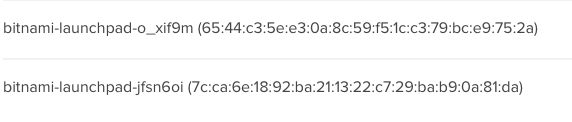
\includegraphics[width=0.5\textwidth]{./03_Analyse/03_Dashboard/images/bitnami_key}
\caption{Bitnami Key}
\end{figure}
Was nicht gerade die Beste Lösung ist.

